\title{Měření v elektrotechnice}

\section{Chyby měření (rozdělení, výpočet, chyby metody, chyby měřicích přístrojů). Nejistoty měření - typy, výpočet nejistoty A, B, kombinovaná a rozšířená nejistota. Nejistoty nepřímých měření.}
Chyba měřění = přesnost prováděného měření, vyjadřuje se jako rozdíl mezi naměřenou a skutečnou hodnotou měřené veličiny.
\subsection*{Rozdělení}
\begin{itemize}
    \item Chyby měření
    \begin{itemize}
        \item Absolutní
        \item Relativní
    \end{itemize}
    \item Chyba metody
    \item Chyba měřícího přístroje
        \begin{itemize}
            \item Třída přesnosti u analogových měřících přístrojů
            \item Základní chyba číslicových měřících přístrojů
        \end{itemize}
    \item Chyby rušivými vlivy
    \item Podle způsobu výskytu
        \begin{itemize}
            \item systematické
            \item náhodné
            \item hrubé
        \end{itemize}
    \item podle místa vzniku
        \begin{itemize}
            \item Chyby metody měření
            \item Chyba měřícího zařazení
            \item Chyba použitých etalonů
        \end{itemize}
    \item podle příčiny vzniku
        \begin{itemize}
            \item Chyby experimentátora
            \item způsobené rušivými vlivy
            \item vliv přístroje na měřený objekt
        \end{itemize}
\end{itemize}
\newpage
\subsection*{Absolutní chyba měření}
rozdíl mezi naměřenou a kovenčně pravou hodnotou
\begin{equation}
    \Delta_X = X_M - X_P \;\;\;\; [X]
\end{equation}
\subsection*{Relativní chyba měření}
chyba vyjádřená v procentech, častější než absolutní
\begin{equation}
    \delta_X = \frac{\Delta_X}{X_M} \;\;\;\; [\%]
\end{equation}
\subsection*{Korekce}
hodnota, která se musí přičíst k naměřené, aby se získala konvenčně správná hodnota
\begin{equation}
    K_X = X_P - X_M = -\Delta_X \;\;\;\; [X]
\end{equation}
\subsection*{Chyba metody}
vzniká tak, že při výpočtu neuvažujem všechny okolní vlivy nebo zjednodušením/zaokrouhlením výpočtu\\
systematická chyba, která lze eliminovat
\subsection*{Chyba měřícího přístroje}
kalibrací se stanovuje korekční křivka\\
výrobce udává absolutní chybu přístroje\\
\paragraph*{Třída přesnosti pro analogové měřící přístroje}
jedná se o chybu udávanou třídou přesnosti přístroje podle normy ČSN EN 60359(0,05;0,1;0,2;0,3;0,5;1;1,5;2;2,5;3;5)\\
Výpočet třídy přesnosti z maximální absolutní chyby $\Delta_{max}$ na rozsahu $X_R$:
\begin{equation}
    \delta_{TP} = \frac{|\Delta_{max}}{X_R}\cdot 100 \;\;\;\; [\%]
\end{equation}
Jeden přístroj může mět víc tříd nepřesnosti pro různé rozsahy\\
\paragraph*{Vyjadřování chyb číslicového přístroje}
dělí se na:
\begin{itemize}
    \item Základní chybu přístroje
    \item Přídavná chyba přístroje
\end{itemize}
\subparagraph*{Základní chyba}
má dvě složky \\
chyba z měřené hodnoty - nedokonalost nastavení měřících prvků - multiplikativní chyba\\
chyba z rozsahu - posunutí nuly, zbytkové napětí - aditivní chyba\\
Absolutní chyba:
\begin{equation}
    |\Delta_p| = |\Delta_M| + |\Delta_R| = \frac{|\delta_M \cdot X_M|+|\delta_R \cdot X_R|}{100}
\end{equation}
index M - naměřená hodnota \\
index R - rozsah \\
Relativní chyba:
\begin{equation}
    |\delta_p| = |\delta_M| + |\delta_R| 
\end{equation}
\\
Způsob zapsání chyby:\\
\textpm(0,05\% z údaje + 0,01\% z rozsahu)\\
\textpm(0,05\% z údaje + 1 digit)
\begin{equation}
    \delta_R = \frac{d}{D}\cdot 100 \;\;\;\;[\%]
\end{equation}
D \dots maximální počet digitů(tj. největší zobrazitelné číslo) \\
d \dots udaný počet digitů posledního místa displeje(většinou 1)\\
\subsection*{Systematické chyby}
přičítá nebo násobí se k měřené hodnotě\\
lze ji určit výpočtem nebo přesnějším měřením\\
lze téměř eliminovat\\

\subsection*{Náhodné chyby}
nelze odstranit korekcí, chová se nepředvídatelně\\
směrodatná odchylka do jisté míry určuje přesnost měření - určuje tvar gaussovy křivky
\begin{equation}
    \sigma = \sqrt{\frac{1}{N}\sum^N_{i=1}(x_i-\overline{x})^2}
\end{equation}
\newpage
\subsection*{Hrubé chyby}
hrubý zásah do procesu měření, výrazně převyšuje rozptyl statistické chyby \\
omyl člověka, výrazná změna podmínek, porucha\\
\begin{figure}[H]
        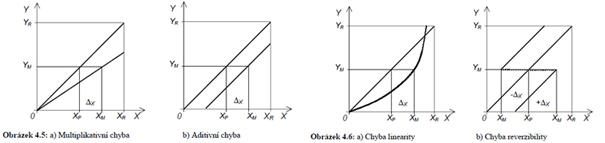
\includegraphics{images/chyby.png}

\end{figure}

\subsection*{Nejistoty}
Parametr přidružený k výsledku měření, který charakterizuje rozptyl hodnot, které by mohly být důvodně přisuzovány k měřené veličině s určitou pravděpodobností.\\
\begin{itemize}
    \item Standartní nejistota typu A
    \item Standartní nejistota typu B 
    \item Kombinovaná standartní nejistota
    \item Rozšířená standartní nejistota
    \item Nejistoty pro nepřímá měření
\end{itemize}

\subsubsection*{Standartní nejistota typu A}
Určuje se  z opakovaných měření.\\
zjišťuje se pomocí výběrového rozptylu hodnot.\\
Mírou nejistoty typu A je výběrový směrodatná odchylka výběrového průměru\\
\begin{equation}
    \overline{x} = \frac{1}{n}\sum^n_{i=1}
\end{equation}
\begin{equation}
    u_a(x) = \sqrt{\frac{1}{n(n-1)}\sum^n_{i=1}(x_i-\overline{x})^2}
\end{equation}
\newpage

\subsubsection*{Standartní nejistota typu B}
Nutnost znát všechny zdroje nejistot, které se dají kvalifikovat, tedy určit jinak, než experimentálně.\\
Zdroje nejistot - kalibrace, stabilita přístrojů, dynamické chyby přístrojů, vnitřní tření\\
Vlivy:
\begin{itemize}
    \item vliv metody - ztráty, interakce s měřeným předmětem, nejistoty použitých konstantn, vlastní ohřev, vlivy reálných parametrů oproti ideálním
    \item vliv operátora - nedodržení metodik, elektrostatické pole, tepelné vyzařování
    \item ostatní vlivy - náhodné omyly při odečtu nbo zápisu hodnot, globální vlivy
\end{itemize}
Dají se vypsat z datasheetů nebo odhadovat.\\
Výpočet nejistoty B:
\begin{equation}
    u_{BZ}(x) = \frac{\Delta_{zmax}}{\kappa}
\end{equation}
Celková nejistota typu B je geometrický součet nejistot jednotlivých zdrojů
\begin{equation}
    u_B(x) = \sqrt{\sum^n_{z=1}u^2_{Bz}(x)}
\end{equation}
Koeficient tvaru rozložení $\kappa$ se určuje z tabulky:
\begin{figure}[H]
    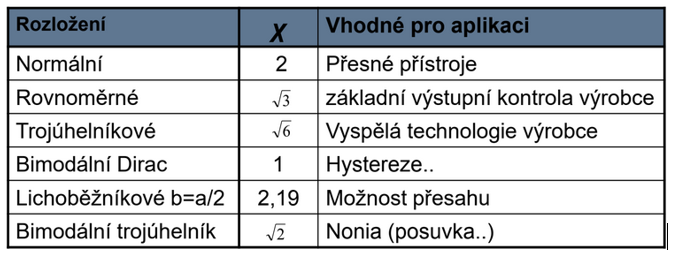
\includegraphics[scale = 1]{images/koef_rozlozeni.png}
\end{figure}
\newpage
Vzorový výpočet nejistoty typu B pro analogový přístroj:
\begin{figure}[H]
    \centering
    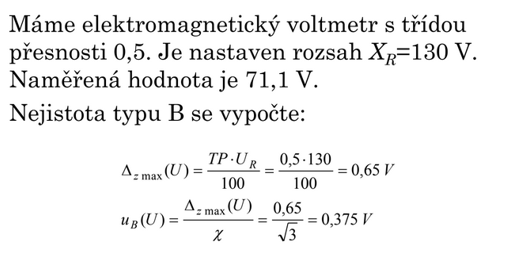
\includegraphics[scale = 1]{images/nejistotaB_analog.png}
\end{figure}
Vzorový výpočet pro nejistotu typu B pro digitální přístroj:
\begin{figure}[H]
    \centering
    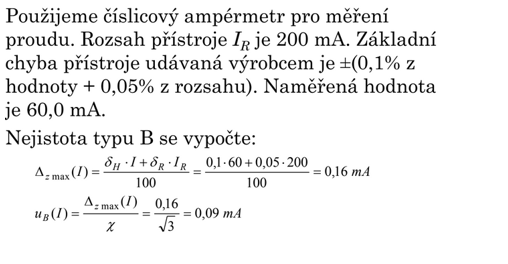
\includegraphics[scale = 1]{images/nejistotaB_digital.png}
\end{figure}

\subsubsection*{Kombinovaná standartní nejistota}
Geometrický součet nejistoty typu A a B 
\begin{equation}
    u_C(x) = \sqrt{u_A^2(x)+u_B^2(x)}
\end{equation}
\newpage

\subsubsection*{Rozšířená standartní nejistota}
Kombinovaná standartní nejistota odpovídá intervalu, ve kterém by se výsledky pohybovaly s pravděpodobností 68\%.\\
Rozšířená standartní nejistota pomocí koeficientu tuto pravděpodobnost zvyšuje, koeficient se volí podle tabulky:
\begin{figure}[H]
    \centering
    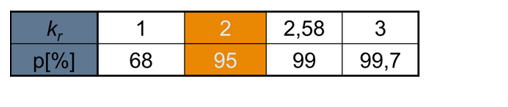
\includegraphics[scale = 1]{images/nejistota_roz.png}
\end{figure}
Nejistota vzniká Kombinovanou standartní nejistotou vynásobenou tímto koeficientem.
\begin{equation}
    U(x) = k_r\cdot u_C(x)
\end{equation}

\subsection*{Nepřímá měření}
Výsledek měření je určen výpočtem na základě známých fyzikálních zákonů z přímých měření vstupních veličin.\\
Výstupní veličina je funkcí průměrných vstupních veličin.\\
\subsubsection*{Nejistota nepřímého měření nekorelovaných vstupních veličin}
Odhad veliiny Y, která je funkcí nekorelovaných vstupních veličin X je dána vztahem:
\begin{equation}
    u(\overline{y}) = \sqrt{\sum^N_{i=1}\left(\frac{\partial f}{\partial X_i}u(\overline{x_i})\right)^2} = \sqrt{\sum^N_{i=1}A_i^2\cdot u^2(\overline{x_i})}
\end{equation}
\begin{equation}
    A_i = \frac{\partial f(X_1,X_2,\dots ,X_N)}{\partial X_i}
\end{equation}
$f$ \dots funkční závislost pro výstupní veličinu $Y$ \\
$A_i$ \dots citlivostní koeficient\\
$u(\overline{x_i})$ \dots nejistota odhadu vstupní veličiny $X_i$\\
\newpage
\subsubsection*{Nejistota nepřímého měření vzájemně korelovaných vstupních veličin}
Odhad veličiny $Y$, která je funkcí vzájemně korelovaných vstupníc veličin $X$, zahrnuje rovněž kovariance mezi jednotlivými odhady vstupních veličin a ty rovněž přispívají k výsledné nejistotě podle vztahu:
\begin{equation}
    u(\overline{y}) = \sqrt{\sum^N_{i=1}A_i^2\cdot u^2(\overline{x_i})+2\sum^N_{i=2}\sum^{N-1}_{k<i}A_i\cdot A_k \cdot u^2(\overline{x_i},\overline{x_k})}
\end{equation}
$u(\overline{x_i},\overline{x_k})$ \dots kovariace mezi navzájem korelovanými odhady vstupních veličin $\overline{x_i},\overline{x_k}$


\section{Analogově-číslicové převoddníky pro měřicí techniku - rozdělení, princip základních typů AD převodníků, vlastnosti, použití}
Převod analogové diskrétní proměnné veličiny(napětí) na diskrétní údaj vyjádřený číslem.\\
Diskretizace analogového signálu:
\begin{itemize}
    \item V amplitudě - kvantování
    \item V čase - vzorkování(vzorkovací teorém - vzorkovací frekvence musí být větší, než 2* maximální požadovaná přenášená frekvence)
    \item Kódování
\end{itemize}
Kvantizační chyba - chyba zaokrouhlování na nejmenší jednotku přístroje. Při časové změně měřené veličiny vzniká kvantovací šum\\
\begin{figure}[H]
    \centering
    \includegraphics*[scale = 1]{images/adc_prevodni_char.png}
    \caption*{Převodní charakteristika měřicího přístroje}
\end{figure}
$K_i$ ideální převodní charakteristika\\
$K_S$ je skutečná převodní charakteristika\\
Chyby, které se vyskytují:
\begin{itemize}
    \item chyba nuly - nenulový výstup pro nulové napětí
    \item chyba konstanty - jiný sklon charakteritiky
    \item chyba linearity - průměrná charakteristika není lineární
\end{itemize}
\newpage
Kritéria hodnocení AD převodníku:
\begin{itemize}
    \item rozlišovací schopnost
    \item krok kvantování
    \item chyba kvantování
    \item rychlost převodu 
    \item přesnost 
    \item stabilita
\end{itemize}
\subsection*{Rozdělení AD převodníků}
\begin{itemize}
    \item Komparační
    \begin{itemize}
        \item Metoda paralelního porovnání
        \item Metoda sérioparalelního porovnání
    \end{itemize}
    \item Kompenzační
    \begin{itemize}
        \item Kompenzační metoda
        \item Metoda postupné aproximace
    \end{itemize}
    \item Integrační
    \begin{itemize}
        \item Integrační metoda (metoda dvojté integrace)
        \item Převod napětí na kmitočet metodou jednoduché integrace 
    \end{itemize}
    \item Sigma-delta modulace
\end{itemize}

\subsection*{Komparační A/D převodník(FLASH)}
Srovnává měřené napětí s různě nastavenýma hodnotama referenčního napětí najednou.\\
Vzorkovací frekvence desítky MHz až 3 GHz\\
krátká doba převodu(ns) - nejrychlejší\\
drahý, není odolný vůči sériovému rušení
\begin{figure}[H]
    \includegraphics*[scale = 1.3]{images/adc_komparacni.png}
\end{figure} 
\newpage
\subsection*{Kompenzační A/D převodník}
měřené konstantní napětí se porovnává se známým stavitelným kompenzačním napětím - nastavuje se tak, aby se blížilo měřenému\\
nejde nastavit naprostá shoda, maximálně zanedbatelný rozdíl - nastavuje se postupně\\
Typy:
\begin{itemize}
    \item Přírůstkový převodník
    \item Sledovací převodník - umožňuje čítat i dolů
    \item Aproximační převodník - nahrazen registrem
\end{itemize}
\subsubsection*{Metoda postupné aproximace}
Hodnota napětí vyjádřena přirozeným binárním číslem\\
při převodu se určuje bit po bitu od největšího po nejmenší\\
8-16 bitové\\
vzorkovací frekvence 10kHz - 3MHz\\
\begin{figure}[H]
    \includegraphics*[scale = 1]{images/adc_kompenzacni_aprox.png}
\end{figure}
\newpage

\subsection*{Integrační A/D převodník}
vhodné a často používané pro číslicové voltmetry\\
výsledkem integrace je střední hodnota\\
Parametry:
\begin{itemize}
    \item 10-27 bitové
    \item vzorkovací frekvence 0,1Hz až 1kHz 
    \item pomalé
    \item velká přesnost, eliminace sériového rušení 
\end{itemize}
Princip:
\begin{itemize}
    \item dvojí(dvoutaktní) integrace
    \item neznámé vstupní napětí porovnáváno s referenčním opačné polarity
    \item po skončení druhého taktu stav čítače hodinových pulsů N udává velikost neznámého napětí
\end{itemize}

\begin{equation}
    N = f_hT_2 = f_hT_1\cdot \frac{U_{vst}}{Z_{REF}} = N_c \cdot \frac{U_{vst}}{Z_{REF}} 
\end{equation}
\begin{figure}[H]
    \includegraphics*[scale = 1]{images/adc_integrac.png}
\end{figure}

\subsubsection*{Převodník napětí na kmitočet}
Převod měřeného napětí na kmitočet a ten pak změřit číslicově.\\
převáděné napětíje trvale připojeno na vstup integrátoru, vyvolává změnu napětí na výstupu integrátoru, které se v komparátoru porovnává s konstantním napětím\\
při překročení hodnoty se změní na opačné výstupní napětí integrátoru\\
kmitočet výstupních impulsů je pak úměrný měřenému napětí
\begin{figure}[H]
    \includegraphics*[scale = 1]{images/adc_V_na_f.png}
\end{figure}
 
\subsection*{Sigma-delta modulace}
Dle taktu Uc vzorkování na komparátor\\
Uo obdelníkové, dle trvání vyšší a nižší hodnoty vyjadřuje Ux\\
dobré rozlišení o na 16 bit při 100kHz, dlouhá odezva
\begin{figure}[H]
    \includegraphics*[scale = 1]{images/adc_sigma_delta_schema.png}
\end{figure}

\begin{figure}[H]
    \includegraphics*[scale = 1]{images/adc_sigma_delta_graf.png}
\end{figure}


\subsection*{Vlastnosti}
\begin{itemize}
    \item Rozlišovací schopnost - dána počtem rozlišitelných úrovní analogového signálu. Pro n-bitový převodník je to $2^n$ úrovní
    \item Krok kvantování(citlivost) - rozdíl dvou hodnot vstupního analogového napětí, kdy nastává přechod od jednoho číslicového výstupu k druhému
    \item Chyba kvantování - maximální rozdíl mezi hodnotou analogové veličiny a hodnotou odpovídající danému ódovanému slovu(obvykle polovina kroku kvantování)
    \item Rychlost převodu 
    \item Přesnost - dána chybou převodníku
    \item Stabilita - vyjadřuje stálost převodníku při působení různých rušivých vlivů
\end{itemize}

\subsection*{Použití}
Zpracování analogových signálů v digitálních přístrojích.